\documentclass[a4paper,10pt]{article}
\usepackage[utf8]{inputenc}
\usepackage[T1]{fontenc}
\usepackage[french]{babel}
\usepackage{paracol}
\usepackage{geometry}
\usepackage{graphicx}
\usepackage{enumitem}
\usepackage{fontawesome}
\usepackage{titlesec}
\usepackage{xcolor}
\usepackage{ragged2e}
\usepackage{ifthen}
\usepackage{hyperref}

% styles file
\usepackage{styles}
% ------ ----

% environment variables
\InputIfFileExists{.env.tex}{}{%
  \InputIfFileExists{.env.example.tex}{}{}%
}
% ----------- ---------

% macros
\newcommand{\contactItem}[3][0.2cm]{%
    #2 & #3 \\[#1]%
}

\newcommand{\formationItem}[2]{%
  \textbf{#1} & {\color{gray}\scriptsize (#2)}\\
}


\newcommand{\langageItem}[2]{
  \textbf{#1} & :\ #2\\
}

\newcommand{\skillItem}[2]{%
  {#1}%
  \ifx&#2&%
    % No second argument provided, do nothing
  \else%
    ~(\textit{#2})%
  \fi
}


\newcommand{\cvEntryDescription}[4]{
    \textbf{#1} \hfill \textbf{#2} \\
    \textit{#3} \\
    \vspace{4pt}
    \begin{itemize}[left=2pt,label={--},nosep]
        \item[] #4
    \end{itemize}
}

\newcommand{\cventryBullet}[3]{
    \textbf{#1} \hfill \textbf{#2} \\
    \begin{itemize}[left=0pt,label={--},nosep]
        #3
    \end{itemize}
}

% ------


\geometry{left=1cm, right=1cm, top=1.5cm, bottom=2cm}
\setlength{\columnsep}{1.5cm}

% title sections
\titleformat{\section}{\Large\bfseries\color{black}}{}{0em}{}[\titlerule]

% Modification des colonnes pour avoir une colonne gauche plus petite
\setcolumnwidth{0.38\textwidth, 0.62\textwidth}

\begin{document}

\pagestyle{empty}

\begin{paracol}{2}
  
% left column
\begin{flushleft}

  % picture
  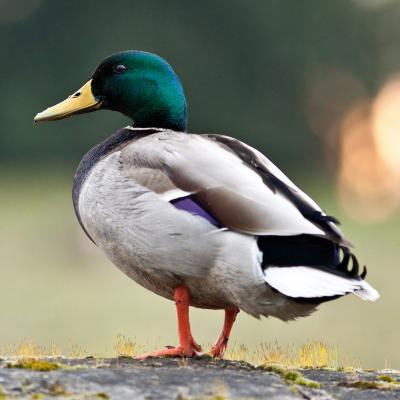
\includegraphics[width=3.3cm]{assets/avatar.jpg} \\[1em]

  \section*{Contact}
  \begin{tabular}{ll}
      \contactItem{\faPhone}{\secretPhoneNumber}
      \contactItem{\faEnvelope}{\secretEmail}
      \contactItem{\faMapMarker}{\secretAddress}
      \contactItem{\faGithub}{\href{https://github.com/Noe-Favier}{Noe-Favier}}
      \contactItem{\faGlobe}{\href{https://noefavier.dev}{noefavier.dev}}
      \contactItem{\faCar}{Permis B}
  \end{tabular}

  \section*{Résumé}
  \begin{justify}
  \hyphenpenalty=10000\exhyphenpenalty=10000\sloppy
  Actuellement en \textbf{fin de Master 2} web, \\
  je suis à la recherche d'un CDI qui me permettra de relever de nouveaux défis et d'explorer de nouveaux horizons professionnels. \\
  Je souhaite mettre mes compétences au service de projets innovants tout en continuant à apprendre et à évoluer dans un milieu social et dynamique.
  \end{justify}

  \section*{Langues}
  \begin{tabular}{ll}
    \langageItem{Français}{Natif}
    \langageItem{TOEIC}{855 / 990 (B2)}
    \langageItem{Espagnol}{A2}
  \end{tabular}

  \section*{Formation}
  \begin{tabular}{ll}
    \formationItem{Master 2 Web Mobile}{en cours}
    \formationItem{Licence Pro DevOps}{2022 - 2023}
    \formationItem{DUT Informatique}{2020 - 2022}
    \formationItem{Bac STI2D, mention TB}{2020}
    \formationItem{BIA aéronautique}{2017}
  \end{tabular}

\end{flushleft}

% right column
\switchcolumn

\begin{flushleft}
  
  {\fontsize{45}{36}\selectfont \textbf{Noé Favier}} \\
  \vspace{0.3em}
  {\Large Alternant en informatique} \\
  \vspace{1em}

  \section*{Compétences}

  \textbf{Frontend}\\
  \skillItem{Angular}{}, \skillItem{Vue3}{}, \skillItem{React}{}, \skillItem{Nuxt}{}, \skillItem{Gatsby}{}, \skillItem{Tailwind}{}, \skillItem{SASS}{}
  
  \vspace{0.5em}
  \textbf{Backend}\\
  \skillItem{Java}{Spring Boot, Wildfly}, \skillItem{PHP}{Symfony}, \skillItem{C\#}{.NET, Blazor}, \skillItem{Rust}{}, \skillItem{Go}{}, \skillItem{Typescript}{Nest}, \skillItem{GraphQL}{}
  
  \vspace{0.5em}
  \textbf{Tooling}\\
  \skillItem{Git}{}, \skillItem{Docker}{}, \skillItem{Kubernetes}{}, \skillItem{Ansible}{}, \skillItem{Terraform}{}, \skillItem{Redis}{}, \skillItem{CI/CD}{GitlabCICD, Github Actions}, \skillItem{PgSQL}{}, \skillItem{Elasticsearch}{}

  \section*{Expériences professionnelles}

  \cvEntryDescription{Alternant développeur analyste}{2022 – 2025 (en cours)}{Axopen, Lyon}{
      Développement web \textbf{java - spring boot} \& \textbf{angular}; missions d'expertise ou devops.
      \begin{itemize}[left=0pt,label={--},nosep]
        \item \textbf{Web} : Création et maintenance d'applications en utilisant des frameworks modernes, contact client.
        \item \textbf{Missions DevOps} : Mise en place de pipelines CI/CD, gestion de conteneurs Docker, installations serveur.
        \item \textbf{Expertise technique} : Audits de code et recommandations d'amélioration.
        \item \textbf{Équipe} : \textbf{Agile} Conception, gestion et \textbf{revue de code} en collaboration avec les membres de l'équipe.
        \item \textbf{Projets} : Implication dans les \textbf{échanges client} pour recueillir les besoins, les traduire en solutions techniques et assurer leur validation. Participation à la gestion de projet agile (suivi, documentation, démonstrations).
      \end{itemize}
    }
  \vspace{1em}
  
  \cventryBullet{Emplois étudiant}{2020 - 2022}{
    Macdonald's \textit{(Salaise, 38150)}, Espaces Verts \textit{(EBER, 38550)}, Rippeur \textit{(EBER, 38550)} \\
  }
  \section*{Projets personnels remarquables}

  \textbf{Filedrop} \hfill \textbf{Rust, Vue3} \\
  Une solution de transfert de fichiers simple et efficace, pensée pour une installation rapide.
  Actuellement en réécriture pour une meilleure interface (vue).
  \begin{itemize}[left=0pt,label={--},nosep]
    \item \textbf{Performances} : écriture en Rust pour une rapidité optimale.
    \item \textbf{Integration} : conteneurisé avec Docker, déployé sur le store de CasaOS.
  \end{itemize}
  \vspace{1em}

  \textbf{DB Drop} \hfill \textbf{Go, Vue3} \\
  Un outil de gestion de base de données sur navigateur, permettant de visualiser et modifier des données de manière intuitive.
  Actuellement en développement, avec une première version fonctionnelle.
  \begin{itemize}[left=0pt,label={--},nosep]
    \item \textbf{Front} : développement en Vue3 pour une interface utilisateur moderne.
    \item \textbf{Back} : utilisation de Go pour une gestion de données efficace.
    \item \textbf{Base de données} : support de PostgreSQL à ce jour, avec des plans d'extension vers d'autres SGBD.
  \end{itemize}
  \vspace{1em}

  \end{flushleft}
  
\end{paracol}

\end{document}